\documentclass[slug=TEM, room=IFW, supervisor=?, coursedate=23.\ 01.\ 2020]{../../Lab_Report_LaTeX/lab_report}

\title{Transmissionselektronenmikroskop}
\author{Oliver Matthes, Valentin Boettcher}
\usepackage{todonotes}
\graphicspath{ {figs/} }
\usepackage{tikz}
\usepackage{pgf}
\usepackage[version=4]{mhchem}
\usepackage[ngerman]{babel}
\usepackage{subcaption}
\usepackage{amssymb}
\usetikzlibrary{external}
\tikzexternalize[prefix=tikz/,optimize command away=\includepdf]

% bib
\addbibresource{protokoll.bib}

\begin{document}
\maketitle

\section{Einleitung}
\label{sec:einl}

Die Transmissionselektronenmikroskopie, kurz TEM, stellt in vielen Bereichen der Natur- und
Ingenieurswissenschaften sowie der Medizin ein wichtiges Verfahren zur Untersuchung von
anorganischen wie organischen Materialien auf deren atomare Struktur oder zur hohen Auflösung
diverser Materialien dar. Man nutzt hierzu Elektronen, da deren geringe Wellenlänge eine
deutlich genauere Auflösung ermöglicht als beispielsweise Röntgenstrahlung und diese einfacher
zu handhaben sind als Gammastrahlung im gleichen Wellenlängenbereich.

\subsection{Aufbau und Funktionsweise eines TEM}
\label{sec:aufbau}

\begin{figure}[h]
	\centering
	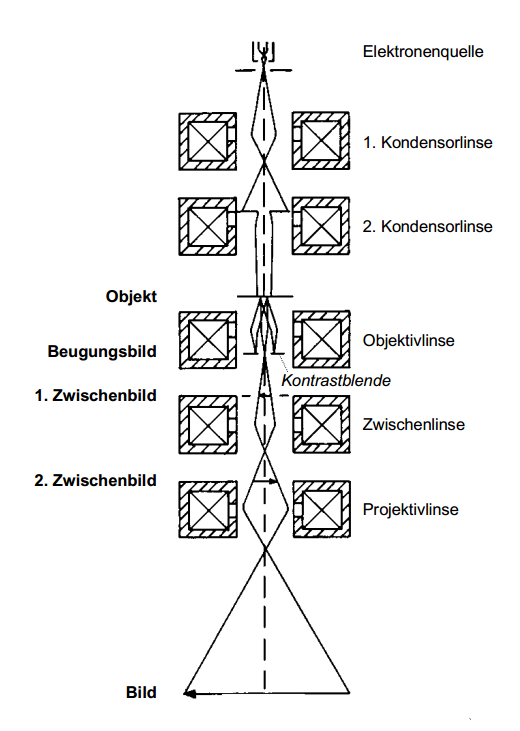
\includegraphics[width=0.5\textwidth]{../protokoll/figures/aufbau_tem.png}
	\caption{Schematische Darstellung des Aufbaus eines TEM mit Skizzierung des Strahlenverlaufs.}
	\label{fig:aufbau}
\end{figure}

In~\ref{fig:aufbau} ist der Aufbau sowie der Strahlenverlauf eines TEM skizziert. Die Elektronen
werden in der Elektronenquelle erzeugt. Dies kann über mehrere verschiedene Verfahren geschehen.

\subsubsection{Elektronenquellen}
\label{sec:equellen}

Die einfachste Möglichkeit, eine Elektronenquelle aufzubauen, ist ähnlich der einer Glühbirne.
Dabei wird eine Wolfram-Haarnadel-Kathode als Emitter genutzt. Um Elektronen zu emittieren, wird
die Kathode erhitzt. Wenige Millimeter hinter der Kathode befindet sich die Wehneltelektrode mit
einem Potential von wenigen \(\SI{-100}{\volt}\). Durch diese Elektrode werden die Elektronen zur
optischen Achse hin gelenkt, sodass ein engster Bündelquerschnitt zwischen Wehneltelektrode und
Anode entsteht. Die Anode sorgt dafür, dass die Elektronen abgesaugt und beschleunigt werden.
Diese Art von Elektronenquellen nennt man wegen der Nutzung allein thermische Anregung zur 
Emission \emph{thermische Elektronenquellen}.\\

Eine andere Möglichkeit stellt die \emph{Feldemissionsquelle} dar, die im Gegensatz zur
rein thermischen Quelle, einen fokussierteren Strahl erzeugen kann. Sie besteht aus einer
sehr dünnen Kathode (Spitzenkathode) mit einer Spitze, die aus Wolframdraht besteht, dessen
Radius ca. \(\SI{50}{\nano\metre}\) groß ist. Die Kathodenspitze ist so dünn damit man starke
elektrische Felder erzeugen kann, um Elektronen allein mit diesen aus der Kathode zu lösen.
Direkt hinter der Kathode befindet sich der Extraktor. Eine Elektrode, die sich auf einem 
Potential von wenigen Kilovolt befindet. Wenn die Elektronen den Extraktor passiert haben werden
sie von der Anode beschleunigt. Bei der Feldemissionsquelle entsteht eine virtuelle Quelle,
die man meist mit Hilfe einer Linse nach der Anode in eine reelle Quelle umwandelt.\\

Eine dritte Möglichkeit ist die Kombination beider Quellarten zur so genannten
\emph{Schottky-Feldemissionsquelle}.

\subsubsection{Magnetische Linsen}
\label{sec:linsen}

Im TEM werden magnetische Rundlinsen verwendet. Diese bestehen aus zwei Spulen, die sich
gegenüber von einander angeordnet sind und in der sich jeweils ein
Kern und an dessen Ende ein Polschuh befinden. Durch die Symmetrie dieser Anordnung wird im
Polschuhspalt ein starkes Magnetfeld (\(\approx \SI{1}{\tesla} \text{bis} \SI{2}{\tesla}\)) 
erzeugt.
Die Variation der Brennweite der Linse erfolgt über eine Variation des Spulenstroms.

\subsubsection{Strahlenverlauf}
\label{sec:verlauf}

Mit Hilfe der Kondensorlinsen, die sich unter der Elektronenquelle befinden kann man die Größe
des bestrahlten Objektbereichs sowie die Beleuchtungsapertur einstellen.
Danach treffen die Elektronen auf das Objekt und werden von diesem entsprechend in ihrem
Verlauf beeinflusst.
In der hinteren Brennebene der Objektivlinsen wird das Beugungsbild erzeugt. Dort werden alle
Elektronen in einem Punkt vereinigt, die im selben Winkel das Objekt verlassen haben.
Nachdem der Strahl die Kontrastblende passiert hat entsteht das erste Zwischenbild. Dabei handelt
es sich bereits um ein Objektbild, das anschließen durch die Zwischen- und Projektivlinse stark
vergrößert und auf einen Leuchtschirm geworfen wird. Dieser Schirm kann hochgeklappt werden, um
zur Aufnahme von Bildern eine CCD-Kamera zu belichten.\\

Im Mikroskop herrscht ein Vakuum damit die Elektronen nicht schon auf ihrem Weg zum oder vom
Objekt an anderen Molekülen gestreut werden und das Objekt an sich nicht Kontaminiert wird. Um zu 
verhindern, dass zum Beispiel durch Eingabe
des Objekts Schmutzmoleküle in das Mikroskop gelangen, wird das Objekt in eine Vakuumschleuse
eingeführt, die vor Eintritt in das Mikroskop ein Vakuum um das Objekt herum herstellt.
Außerdem wird ein Kondensring im Mikroskop mit flüssigem Stickstoff gekühlt, damit eventuelle
störende Moleküle, an diesem kondensieren. NOCHMAL NACHSCHAUEN!

\subsection{Streuung von Elektronen}
\label{sec:streuung}

\subsubsection{Elastische Streuung}
\label{sec:elast}

Von elastische Streuung spricht man, wenn die kinetische Energie des Elektrons vor und nach dem
Stoß gleich bleibt. Dabei wird ein Atom durch das Coulombpotential, das sich aus Atomkern und den
ihn umgebenden, abschirmend wirkenden Elektronen zusammensetzt.

\section{Durchf\"uhrung und Auswertung}
\label{sec:durchaus}

\subsection{Hochaufgel\"oste Abbildung von Goldinseln}
\label{sec:hrtem}

Das TEM wurde im realbildmodus

\newpage
\section{Verzeichnisse}
\label{sec:literatur}

\listoffigures

\listoftables

\printbibliography
\end{document}
